% Application Layer
\documentclass[12pt]{article}
\usepackage[utf8]{inputenc}
\usepackage{amsmath, amssymb}
\usepackage{xcolor}
\usepackage{geometry}
\usepackage{hyperref}
\usepackage{fancyhdr}
\usepackage{enumitem}
\usepackage{minted}
\usepackage{booktabs}
\usepackage{graphicx}
\usepackage{tikz}
\usetikzlibrary{shapes, arrows, positioning}

\geometry{margin=1in}
\hypersetup{colorlinks=true, linkcolor=blue, urlcolor=cyan}

\newcommand{\TOPICTITLE}{Application Layer}

\pagestyle{fancy}
\fancyhf{}
\fancyhead[L]{\textbf{\TOPICTITLE}}
\fancyhead[R]{\thepage}

% -------------------------------
% Topic Metadata
% -------------------------------
\title{\TOPICTITLE\\\large Study-Ready Notes}
\author{Compiled by Andrew Photinakis}
\date{\today}

\setlength{\headheight}{15pt}

\begin{document}
\maketitle
\tableofcontents
\newpage

\documentclass[12pt]{article}
\usepackage[utf8]{inputenc}
\usepackage{amsmath, amssymb}
\usepackage{xcolor}
\usepackage{geometry}
\usepackage{hyperref}
\usepackage{fancyhdr}
\usepackage{enumitem}
\usepackage{minted}
\usepackage{booktabs}
\usepackage{graphicx}
\usepackage{tikz}
\usepackage{caption}
\usetikzlibrary{shapes, arrows, positioning}

% -------------------------------
% Page and link settings
% -------------------------------
\geometry{margin=1in}
\hypersetup{
    colorlinks=true,
    linkcolor=blue,
    urlcolor=cyan
}

% -------------------------------
% Custom Commands & Metadata
% -------------------------------
\newcommand{\TOPICTITLE}{Application Layer - Computer Networks}

\pagestyle{fancy}
\fancyhf{}
\fancyhead[L]{\textbf{\TOPICTITLE}}
\fancyhead[R]{\thepage}
\setlength{\headheight}{15pt}

\title{\TOPICTITLE\\\large Study-Ready Notes}
\author{Compiled by Andrew Photinakis}
\date{\today}

% -------------------------------
% Begin Document
% -------------------------------
\begin{document}

\maketitle
\tableofcontents
\newpage

\section*{Keywords}
\noindent\textbf{Keywords:}
\begin{itemize}
    \item Application Layer
    \item Network Applications
    \item Client-Server Paradigm
    \item Peer-to-Peer (P2P) Architecture
    \item Processes and Sockets
    \item Port Numbers
    \item Application-Layer Protocols
    \item HTTP (Hypertext Transfer Protocol)
    \item SMTP (Simple Mail Transfer Protocol)
    \item IMAP (Internet Message Access Protocol)
    \item DNS (Domain Name System)
    \item Transport Layer Services
    \item TCP (Transmission Control Protocol)
    \item UDP (User Datagram Protocol)
    \item Data Integrity
    \item Throughput Requirements
    \item Timing Constraints
    \item TLS (Transport Layer Security)
    \item Socket Programming
    \item CDNs (Content Delivery Networks)
    \item Video Streaming
    \item Network Security
    \item Protocol Design
\end{itemize}

\section{Application Layer Overview}

\subsection{Overview}
Goal of this is to introduce the application layer of the Internet protocol stack: its goals, common application-layer protocols such as HTTP, SMTP/IMAP, DNS, P2P, streaming/CDNs, and practical programming considerations (socket API, UDP/TCP).
Here we'll contrast application-level requirements with transport services (TCP vs UDP) and touches on security (TLS).


\subsection{Learning Objectives}
\begin{itemize}
    \item Understand conceptual and implementation aspects of application-layer protocols
    \item Study transport-layer service models
    \item Learn client-server and peer-to-peer paradigms
    \item Examine popular application-layer protocols:
          \begin{itemize}
              \item HTTP (Web)
              \item SMTP, IMAP (Email)
              \item DNS (Domain Name System)
          \end{itemize}
    \item Study video streaming systems and CDNs
    \item Learn socket programming with UDP and TCP
\end{itemize}

\textcolor{blue}{[Summary: The application layer focuses on network applications, their protocols, and how they use underlying transport services. Key paradigms include client-server and P2P architectures.]}

\section{Network Applications and Paradigms}

\subsection{Common Network Applications}
\begin{itemize}
    \item Social networking
    \item Web browsing
    \item Text messaging
    \item Email
    \item Multi-user network games
    \item Streaming stored video (YouTube, Hulu, Netflix)
    \item P2P file sharing
    \item Voice over IP (Skype)
    \item Real-time video conferencing (Zoom)
    \item Internet search
    \item Remote login
\end{itemize}

\textcolor{orange}{[Mnemonic: WESTS - Web, Email, Streaming, Texting, Social - covers major application categories]}

\subsection{Creating Network Applications}
\begin{itemize}
    \item Programs run on different end systems
    \item Communication occurs over network
    \item Example: web server software communicates with browser software
    \item \textbf{Key Insight}: No need to write software for network-core devices
          \begin{itemize}
              \item Network-core devices don't run user applications
              \item Applications reside only on end systems
              \item Enables rapid application development and propagation
          \end{itemize}
\end{itemize}

\begin{figure}[h]
    \centering
    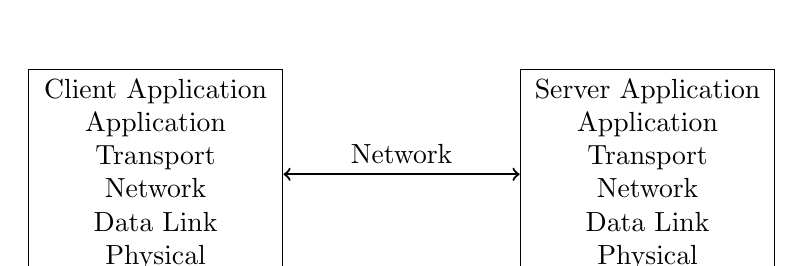
\begin{tikzpicture}[node distance=1.5cm]
        \node (client) [rectangle, draw, text width=3cm, text centered] {Client Application\\Application\\Transport\\Network\\Data Link\\Physical};
        \node (server) [rectangle, draw, text width=3cm, text centered, right=3cm of client] {Server Application\\Application\\Transport\\Network\\Data Link\\Physical};
        \draw [<->, thick] (client.east) -- node[above] {Network} (server.west);
    \end{tikzpicture}
    \caption{Network Application Architecture: Applications run on end systems using the protocol stack}
    \label{fig:network-arch}
\end{figure}

\subsection{Client-Server Paradigm}


\begin{itemize}
    \item \textbf{Server}:
          \begin{itemize}
              \item Always-on host
              \item Permanent IP address
              \item Waits for and serves client requests
          \end{itemize}
    \item \textbf{Clients}:
          \begin{itemize}
              \item Contact and communicate with server
              \item May be intermittently connected
              \item May have dynamic IP addresses
              \item Do not communicate directly with each other
          \end{itemize}
    \item \textbf{Examples}: HTTP, IMAP, FTP
\end{itemize}

\textcolor{blue}{[Summary: Client-server model features dedicated servers that are always available and multiple clients that initiate connections. This is the foundation of most traditional web services.]}

\subsection{Peer-to-Peer (P2P) Architecture}

\begin{itemize}
    \item No always-on server
    \item Arbitrary end systems directly communicate
    \item Peers both request and provide services
    \item \textbf{Key Advantages}:
          \begin{itemize}
              \item Self-scalability: New peers bring new service capacity
              \item Distributed nature reduces single points of failure
          \end{itemize}
    \item \textbf{Challenges}:
          \begin{itemize}
              \item Peers are intermittently connected
              \item Peers change IP addresses
              \item Complex management and coordination
          \end{itemize}
    \item \textbf{Example}: P2P file sharing (BitTorrent)
\end{itemize}

\begin{figure}[h]
    \centering
    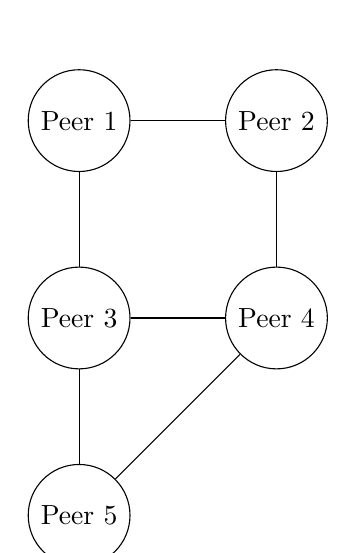
\begin{tikzpicture}[node distance=1.2cm]
        \node (peer1) [circle, draw] {Peer 1};
        \node (peer2) [circle, draw, right=of peer1] {Peer 2};
        \node (peer3) [circle, draw, below=of peer1] {Peer 3};
        \node (peer4) [circle, draw, right=of peer3] {Peer 4};
        \node (peer5) [circle, draw, below=of peer3] {Peer 5};

        \draw (peer1) -- (peer2);
        \draw (peer1) -- (peer3);
        \draw (peer2) -- (peer4);
        \draw (peer3) -- (peer4);
        \draw (peer3) -- (peer5);
        \draw (peer4) -- (peer5);
    \end{tikzpicture}
    \caption{P2P Architecture: Peers connect directly to each other in a mesh network}
    \label{fig:p2p-arch}
\end{figure}

\textcolor{teal}{[Concept Map: Application Architectures → Client-Server (centralized, reliable) vs P2P (decentralized, scalable) → Hybrid approaches combine both]}

\section{Process Communication and Sockets}

\subsection{Processes Communicating}
\begin{itemize}
    \item \textbf{Process}: Program running within a host
    \item \textbf{Client process}: Process that initiates communication
    \item \textbf{Server process}: Process that waits to be contacted
    \item Processes on same host use inter-process communication (IPC)
    \item Processes on different hosts communicate by exchanging messages
    \item Note: P2P applications have both client and server processes
\end{itemize}

\subsection{Sockets}
\begin{itemize}
    \item Process sends/receives messages to/from its socket
    \item \textbf{Analogy}: Socket is like a door
          \begin{itemize}
              \item Sending process shoves message out the door
              \item Transport infrastructure delivers message to receiving process's socket
          \end{itemize}
    \item Two sockets involved: one on each communicating process
    \item \textbf{Developer Control}: Application developer controls application layer
    \item \textbf{OS Control}: Operating system controls transport layer and below
\end{itemize}

\begin{figure}[h]
    \centering
    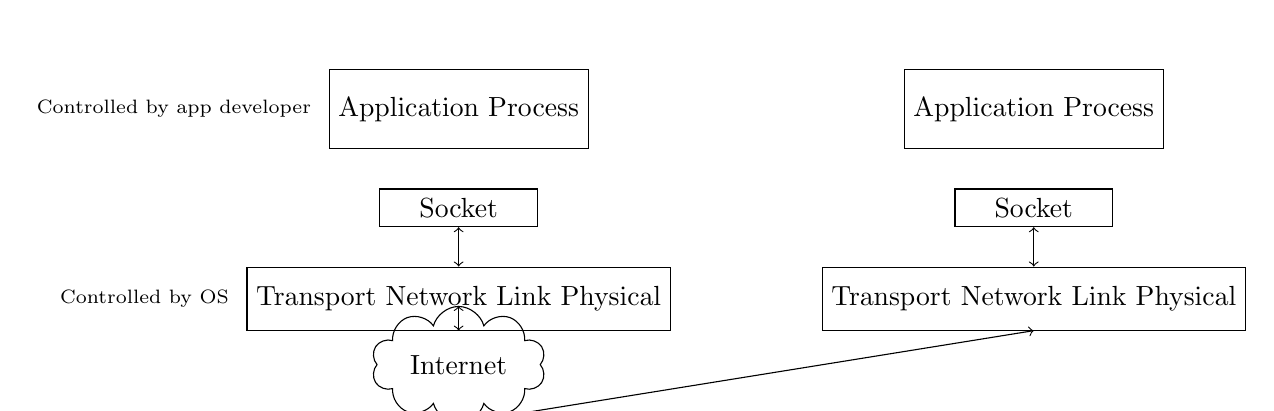
\begin{tikzpicture}[node distance=1.5cm]
        \node (app1) [rectangle, draw, minimum width=3cm, minimum height=1cm] {Application Process};
        \node (socket1) [rectangle, draw, below=0.5cm of app1, minimum width=2cm] {Socket};
        \node (transport1) [rectangle, draw, below=0.5cm of socket1, minimum width=3cm, minimum height=0.8cm] {Transport Network Link Physical};

        \node (app2) [rectangle, draw, minimum width=3cm, minimum height=1cm, right=4cm of app1] {Application Process};
        \node (socket2) [rectangle, draw, below=0.5cm of app2, minimum width=2cm] {Socket};
        \node (transport2) [rectangle, draw, below=0.5cm of socket2, minimum width=3cm, minimum height=0.8cm] {Transport Network Link Physical};

        \node (internet) [cloud, draw, aspect=2, below=1cm of socket1] {Internet};

        \draw [<->] (socket1.south) -- (transport1.north);
        \draw [<->] (socket2.south) -- (transport2.north);
        \draw [<->] (transport1.south) -- (internet.north);
        \draw [<->] (transport2.south) -- (internet.south);

        \node [left=0.1cm of app1] {\scriptsize Controlled by app developer};
        \node [left=0.1cm of transport1] {\scriptsize Controlled by OS};
    \end{tikzpicture}
    \caption{Socket Communication: Applications use sockets as interface to network services}
    \label{fig:socket-comm}
\end{figure}

\subsection{Addressing Processes}
\begin{itemize}
    \item To receive messages, process must have an identifier
    \item Host has unique 32-bit IP address
    \item IP address alone is insufficient - many processes can run on same host
    \item Complete identifier includes: IP address + port numbers
    \item \textbf{Common Port Numbers}:
          \begin{itemize}
              \item HTTP server: port 80
              \item Mail server: port 25
              \item Example: Sending HTTP to gaia.cs.umass.edu
                    \begin{itemize}
                        \item IP address: 128.119.245.12
                        \item Port number: 80
                    \end{itemize}
          \end{itemize}
\end{itemize}

\textcolor{blue}{[Summary: Processes communicate through sockets, which act as endpoints. Addressing requires both IP address and port number to uniquely identify applications on hosts.]}

\section{Application-Layer Protocols}

\subsection{Protocol Definition}
An application-layer protocol defines:
\begin{itemize}
    \item \textbf{Types of messages exchanged}: Request, response messages
    \item \textbf{Message syntax}: Fields and how they are delineated
    \item \textbf{Message semantics}: Meaning of information in fields
    \item \textbf{Rules}: When and how processes send and respond to messages
\end{itemize}

\subsection{Protocol Types}
\begin{itemize}
    \item \textbf{Open Protocols}:
          \begin{itemize}
              \item Defined in RFCs (Request for Comments)
              \item Everyone has access to protocol definition
              \item Enables interoperability
              \item Examples: HTTP, SMTP
          \end{itemize}
    \item \textbf{Proprietary Protocols}:
          \begin{itemize}
              \item Privately owned and controlled
              \item May provide competitive advantages
              \item Examples: Skype, Zoom
          \end{itemize}
\end{itemize}

\textcolor{orange}{[Mnemonic: SSTR - Syntax, Semantics, Timing, Rules - the four components of protocols]}

\section{Transport Service Requirements}

\subsection{Application Needs}
Different applications have different transport service requirements:
\begin{itemize}
    \item \textbf{Data Integrity}:
          \begin{itemize}
              \item Some apps require 100\% reliable data transfer (file transfer, web transactions)
              \item Other apps can tolerate some loss (audio)
          \end{itemize}
    \item \textbf{Throughput}:
          \begin{itemize}
              \item Some apps require minimum throughput (multimedia)
              \item Other apps are elastic (use whatever throughput available)
          \end{itemize}
    \item \textbf{Timing}:
          \begin{itemize}
              \item Some apps require low delay (Internet telephony, interactive games)
          \end{itemize}
    \item \textbf{Security}: Encryption, data integrity, authentication
\end{itemize}

\subsection{Common Application Requirements}

\begin{table}[h]
    \centering
    \begin{tabular}{p{4cm}ccc}
        \toprule
        \textbf{Application}   & \textbf{Data Loss} & \textbf{Throughput} & \textbf{Time Sensitive?} \\
        \midrule
        File transfer/download & No loss            & Elastic             & No                       \\
        E-mail                 & No loss            & Elastic             & No                       \\
        Web documents          & No loss            & Elastic             & No                       \\
        Real-time audio/video  & Loss-tolerant      & Audio: 5Kbps-1Mbps                             \\Video: 10Kbps-5Mbps & Yes, 10's msec \\
        Streaming audio/video  & Loss-tolerant      & Same as above       & Yes, few secs            \\
        Interactive games      & Loss-tolerant      & Kbps+               & Yes, 10's msec           \\
        Text messaging         & No loss            & Elastic             & Yes and no               \\
        \bottomrule
    \end{tabular}
    \caption{Transport Service Requirements for Common Applications}
    \label{tab:app-requirements}
\end{table}

\textcolor{blue}{[Summary: Applications have varying requirements for data integrity, throughput, and timing. Real-time applications tolerate some loss but need low delay, while data transfer applications require reliability but can tolerate delay.]}

\section{Internet Transport Protocols}

\subsection{TCP Service}
\begin{itemize}
    \item \textbf{Reliable transport} between sending and receiving process
    \item \textbf{Flow control}: Prevents sender from overwhelming receiver
    \item \textbf{Congestion control}: Throttles sender when network overloaded
    \item \textbf{Connection-oriented}: Setup required between client and server
    \item \textbf{Does not provide}: Timing, minimum throughput guarantee, security
\end{itemize}

\subsection{UDP Service}
\begin{itemize}
    \item \textbf{Unreliable data transfer} between processes
    \item \textbf{Does not provide}: Reliability, flow control, congestion control, timing, throughput guarantee, security, or connection setup
\end{itemize}

\textbf{Q: Why bother with UDP? Why is there a UDP?}
\begin{itemize}
    \item Lower overhead than TCP
    \item No connection establishment delay
    \item Simpler header and no congestion control overhead
    \item Suitable for applications that can tolerate some loss but need low latency
    \item Applications can implement their own reliability if needed
\end{itemize}

\subsection{Applications and Transport Protocols}

\begin{table}[h]
    \centering
    \begin{tabular}{p{4cm}p{4cm}p{3cm}}
        \toprule
        \textbf{Application}   & \textbf{Application Layer Protocol}            & \textbf{Transport Protocol} \\
        \midrule
        File transfer/download & FTP [RFC 959]                                  & TCP                         \\
        E-mail                 & SMTP [RFC 5321]                                & TCP                         \\
        Web documents          & HTTP 1.1 [RFC 7320]                            & TCP                         \\
        Internet telephony     & SIP [RFC 3261], RTP [RFC 3550], or proprietary & TCP or UDP                  \\
        Streaming audio/video  & HTTP [RFC 7320], DASH                          & TCP                         \\
        Interactive games      & WOW, FPS (proprietary)                         & UDP or TCP                  \\
        \bottomrule
    \end{tabular}
    \caption{Internet Applications and Their Protocols}
    \label{tab:app-protocols}
\end{table}

\textcolor{teal}{[Concept Map: Transport Protocols → TCP (reliable, connection-oriented) vs UDP (unreliable, connectionless) → Application choice depends on reliability vs latency requirements]}

\section{Transport Layer Security (TLS)}

\subsection{Security in TCP/UDP}
\begin{itemize}
    \item \textbf{Vanilla TCP \& UDP sockets}: No encryption
    \item Cleartext passwords sent into socket traverse Internet in cleartext
    \item Major security vulnerability
\end{itemize}

\subsection{Transport Layer Security (TLS)}
\begin{itemize}
    \item Provides encrypted TCP connections
    \item Ensures data integrity
    \item Provides end-point authentication
    \item TLS is implemented in application layer
    \item Applications use TLS libraries, which use TCP in turn
    \item Cleartext sent into "socket" traverses Internet encrypted
\end{itemize}

\textcolor{blue}{[Summary: TLS provides security for TCP connections by adding encryption, data integrity, and authentication. It's implemented at the application layer but provides transport-layer security services.]}

\section{Course Topics Overview}

\subsection{Application Layer Coverage}
The course will cover:
\begin{itemize}
    \item Principles of network applications
    \item Web and HTTP
    \item E-mail, SMTP, IMAP
    \item The Domain Name System: DNS
    \item P2P applications
    \item Video streaming, CDNs
    \item Socket programming with UDP and TCP
\end{itemize}

\textcolor{orange}{[Mnemonic: WED P2P VS - Web, Email, DNS, P2P, Video Streaming - major application layer topics]}

\section{Exam Questions}

\subsection*{Application Layer Fundamentals}
\begin{enumerate}
    \item Compare and contrast client-server and peer-to-peer architectures. What are the advantages and disadvantages of each?
    \item Explain why network applications are written to run on end systems rather than network core devices.
    \item Describe the role of sockets in network communication. What aspects are controlled by the application developer versus the operating system?
\end{enumerate}

\subsection*{Transport Protocols}
\begin{enumerate}
    \item What are the key differences between TCP and UDP? For what types of applications would you choose each and why?
    \item Explain why some applications can tolerate packet loss while others require 100\% reliability. Provide examples of each type.
    \item How does TLS enhance the security of TCP connections? At what layer is TLS implemented?
\end{enumerate}

\subsection*{Protocol Design}
\begin{enumerate}
    \item What four key elements does an application-layer protocol define? Provide examples for each element using HTTP.
    \item Explain the difference between open protocols and proprietary protocols. What are the benefits of each approach?
    \item Why is both an IP address and port number needed to identify a process running on a host?
\end{enumerate}

\textcolor{red}{[Exam Questions: Focus on comparing architectures, understanding transport protocol trade-offs, and analyzing application requirements. Practice explaining concepts with concrete examples.]}


\section{Textbook Chapter}
\section{2.1.1 Network Application Architectures}
\begin{enumerate}
    \item From the application developer’s perspective, the network architecture is fixed and provides a specific set of services to applications.
    \item When choosing an application architecture, an app dev will likely choose either client-server or peer-to-peer.
    \item The choice of architecture impacts scalability, performance, and complexity of the application.
\end{enumerate}


\end{document}
\documentclass[12pt]{article}
\usepackage[utf8]{inputenc}
\usepackage{amsmath, amssymb}
\usepackage{xcolor}
\usepackage{geometry}
\usepackage{hyperref}
\usepackage{fancyhdr}
\usepackage{enumitem}
\usepackage{minted}
\usepackage{booktabs}
\usepackage{tikz} 
\usetikzlibrary{positioning}


\geometry{margin=1in}
\hypersetup{colorlinks=true, linkcolor=blue, urlcolor=cyan}

\pagestyle{fancy}
\fancyhf{}
\fancyhead[L]{\textbf{\TOPICTITLE}}
\fancyhead[R]{\thepage}

% -------------------------------
% Topic Metadata
% -------------------------------
\newcommand{\TOPICTITLE}{Application Layer: Web and HTTP}
\title{\TOPICTITLE\\\large Study-Ready Notes}
\author{Compiled by Andrew Photinakis}
\date{\today}

\setlength{\headheight}{15pt}

\begin{document}
\maketitle
\tableofcontents
\newpage

\section*{Keywords}
\noindent\textbf{Keywords:}
\begin{itemize}
    \item Application Layer
    \item Network Applications
    \item Client-Server Paradigm
    \item Peer-to-Peer (P2P) Architecture
    \item Processes and Sockets
    \item Port Numbers
    \item Application-Layer Protocols
    \item HTTP (Hypertext Transfer Protocol)
    \item SMTP (Simple Mail Transfer Protocol)
    \item IMAP (Internet Message Access Protocol)
    \item DNS (Domain Name System)
    \item Transport Layer Services
    \item TCP (Transmission Control Protocol)
    \item UDP (User Datagram Protocol)
    \item Data Integrity
    \item Throughput Requirements
    \item Timing Constraints
    \item TLS (Transport Layer Security)
    \item Socket Programming
    \item CDNs (Content Delivery Networks)
    \item Video Streaming
    \item Network Security
    \item Protocol Design
\end{itemize}



\section{Introduction to Application Layer}
\begin{itemize}
    \item Principles of network applications
    \item Web and HTTP (part 1 and 2)
    \item E-mail, SMTP, IMAP
    \item The Domain Name System: DNS
    \item P2P applications
    \item Video streaming, CDNs
    \item Socket programming with UDP and TCP
\end{itemize}

\textcolor{blue}{[Summary: The application layer is the top layer in network protocols, handling user-facing services like web browsing, email, and file transfer. It defines how applications communicate over networks.]}

\section{Web and HTTP Fundamentals}

\subsection{Web Page Composition}
\begin{itemize}
    \item Web pages consist of multiple \textbf{objects}
    \item Each object can be stored on different web servers
    \item Objects can be: HTML files, JPEG images, Java applets, audio files, etc.
    \item Base HTML file includes references to other objects
    \item Each object is addressable by a \textbf{URL}
\end{itemize}

\textbf{URL Structure:}
\begin{verbatim}
www.someschool.edu/someDept/pic.gif
|              |   |
host name      |   path name
              domain
\end{verbatim}

\subsection{HTTP Overview}
\begin{itemize}
    \item \textbf{HTTP:} Hypertext Transfer Protocol
    \item Web's application-layer protocol
    \item Uses \textbf{client/server model}:
          \begin{itemize}
              \item \textbf{Client:} Browser that requests, receives, and displays web objects
              \item \textbf{Server:} Web server that sends objects in response to requests
          \end{itemize}
\end{itemize}

\begin{figure}[h]
    \centering
    \begin{tabular}{c c c}
        PC running      & $\rightarrow$           & Server running    \\
        Firefox browser & HTTP requests/responses & Apache Web server \\
        iPhone running  & $\rightarrow$           &                   \\
        Safari browser  & HTTP requests/responses &                   \\
    \end{tabular}
    \caption{HTTP Client-Server Architecture}
\end{figure}

\textcolor{blue}{[Summary: HTTP is the foundation of web communication, using a client-server model where browsers request resources and servers provide them.]}

\section{HTTP Connections}

\subsection{Connection Types}
\begin{itemize}
    \item \textbf{Non-persistent HTTP:}
          \begin{enumerate}
              \item TCP connection opened
              \item At most one object sent over TCP connection
              \item TCP connection closed
              \item Downloading multiple objects requires multiple connections
          \end{enumerate}

    \item \textbf{Persistent HTTP:}
          \begin{itemize}
              \item TCP connection opened to a server
              \item Multiple objects can be sent over \textit{single} TCP connection
              \item TCP connection closed after all objects transferred
          \end{itemize}
\end{itemize}

\subsection{Non-persistent HTTP Example}
\textbf{Scenario:} User enters URL: www.someSchool.edu/someDepartment/home.index (contains text + 10 JPEG references)

\begin{enumerate}
    \item HTTP client initiates TCP connection to HTTP server on port 80
    \item HTTP client sends HTTP request message with URL
    \item HTTP server receives request, forms response with requested object
    \item HTTP server closes TCP connection
    \item HTTP client receives response, displays HTML, finds 10 referenced JPEGs
    \item Steps 1-5 repeated for each of 10 JPEG objects
\end{enumerate}

\subsection{Response Time Analysis}
\begin{itemize}
    \item \textbf{RTT (Round Trip Time):} Time for small packet to travel from client to server and back
    \item \textbf{Non-persistent HTTP Response Time:}
          \[ \text{Response Time} = 2 \times \text{RTT} + \text{File Transmission Time} \]
          \begin{itemize}
              \item One RTT to initiate TCP connection
              \item One RTT for HTTP request and first bytes of response
              \item Object/file transmission time
          \end{itemize}
\end{itemize}

\begin{figure}[h]
    \centering
    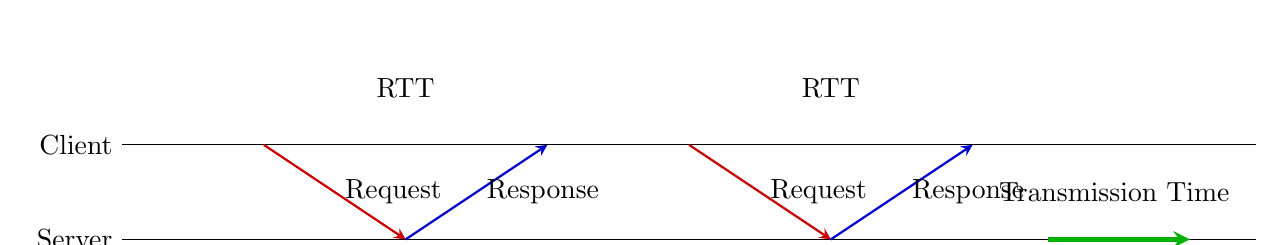
\begin{tikzpicture}[scale=1.2, >=stealth]
        % Client and Server lines
        \draw (0,1) -- (12,1);
        \draw (0,0) -- (12,0);
        \node[left] at (0,1) {Client};
        \node[left] at (0,0) {Server};

        % RTT 1 (Request + Response)
        \draw[->, thick, color=red!80!black] (1.5,1) -- (3,0)
        node[midway, right, black] {Request};
        \draw[->, thick, color=blue!80!black] (3,0) -- (4.5,1)
        node[midway, right, black] {Response};
        \node[above] at (3,1.4) {RTT};

        % RTT 2 (Request + Response)
        \draw[->, thick, color=red!80!black] (6,1) -- (7.5,0)
        node[midway, right, black] {Request};
        \draw[->, thick, color=blue!80!black] (7.5,0) -- (9,1)
        node[midway, right, black] {Response};
        \node[above] at (7.5,1.4) {RTT};

        % Transmission Time
        \draw[->, ultra thick, color=green!70!black] (9.8,0) -- (11.3,0);
        \node[above, black] at (10.5,0.3) {Transmission Time};
    \end{tikzpicture}
    \caption{Non-persistent HTTP Response Time Components (colored by message type)}
    \label{fig:http_rtt}
\end{figure}

\textcolor{orange}{[Mnemonic: Non-persistent = "One and Done" - one object per connection]}
\textcolor{blue}{[Summary: Non-persistent HTTP requires separate connections for each object, leading to 2 RTTs per object, while persistent HTTP reuses connections for multiple objects.]}

\section{Persistent HTTP (HTTP 1.1)}

\subsection{Non-persistent HTTP Issues}
\begin{itemize}
    \item Requires 2 RTTs per object
    \item OS overhead for each TCP connection
    \item Browsers open multiple parallel TCP connections to fetch objects
\end{itemize}

\subsection{Persistent HTTP Advantages}
\begin{itemize}
    \item Server leaves connection open after sending response
    \item Subsequent HTTP messages use same connection
    \item Client sends requests immediately upon encountering referenced objects
    \item As little as one RTT for all referenced objects
    \item Cuts response time in half compared to non-persistent
\end{itemize}

\textcolor{teal}{[Concept Map:
            \begin{itemize}
                \item HTTP 1.0 → Non-persistent → Multiple connections → High overhead
                \item HTTP 1.1 → Persistent → Single connection → Lower overhead
                \item Performance improvement: 2RTT/object → ~1RTT/multiple objects
            \end{itemize}
        ]}

\section{HTTP Message Format}

\subsection{HTTP Request Message}
\begin{itemize}
    \item ASCII (human-readable format)
    \item Two types: request and response messages
\end{itemize}

\textbf{General Format:}
\begin{verbatim}
| method | sp | URL | sp | version | cr | lf |
| header field name | : | value | cr | lf |
| ... |
| cr | lf |
| entity body |
\end{verbatim}

\subsection{HTTP Request Methods}
\begin{itemize}
    \item \textbf{GET:} Request object from server
          \begin{itemize}
              \item Can include user data in URL after '?': www.sombsite.com/animalsearch?monkeys\&banana
          \end{itemize}

    \item \textbf{POST:} Send data to server
          \begin{itemize}
              \item Used for form input
              \item User input sent in entity body
          \end{itemize}

    \item \textbf{HEAD:} Request headers only (no body)
    \item \textbf{PUT:} Upload new file to server
          \begin{itemize}
              \item Completely replaces existing file
          \end{itemize}
\end{itemize}

\subsection{HTTP Response Message}
\begin{itemize}
    \item \textbf{Status line:} protocol + status code + status phrase
    \item Example: HTTP/1.1 200 OK
\end{itemize}

\subsection{HTTP Response Status Codes}
\begin{itemize}
    \item \textbf{200 OK:} Request succeeded, object in message
    \item \textbf{301 Moved Permanently:} Object moved, new location specified
    \item \textbf{400 Bad Request:} Request not understood
    \item \textbf{404 Not Found:} Requested document not found
    \item \textbf{505 HTTP Version Not Supported:} Unsupported protocol version
\end{itemize}

\textcolor{blue}{[Summary: HTTP messages follow specific formats with request methods (GET, POST, HEAD, PUT) and response codes (200, 301, 404, etc.) that indicate request outcomes.]}

\section{HTTP in Practice}

\subsection{Trying HTTP with Netcat}
\begin{enumerate}
    \item Open TCP connection: \texttt{\% nc -c -v cs.rit.edu 80}
    \item Send GET request:
          \begin{verbatim}
    GET interactive/index.php HTTP/1.1
    Host: cs.rit.edu
    \end{verbatim}
    \item Examine server response
\end{enumerate}

\subsection{HTTP State Management: Cookies}
\begin{itemize}
    \item HTTP is \textbf{stateless} - no memory between requests
    \item \textbf{Cookies} maintain state between transactions
\end{itemize}

\textbf{Four Cookie Components:}
\begin{enumerate}
    \item Cookie header line in HTTP \textit{response} message
    \item Cookie header line in HTTP \textit{request} message
    \item Cookie file on user's host (managed by browser)
    \item Back-end database at website
\end{enumerate}

\begin{figure}[h]
    \centering
    \begin{tabular}{c c c}
        Client       &                  & Server              \\
        Cookie file  & $\rightarrow$    & Backend database    \\
        Amazon: 1678 & HTTP with cookie & ID: 1678, user data \\
    \end{tabular}
    \caption{Cookie-based State Management}
\end{figure}

\begin{figure}[h]
    \centering
    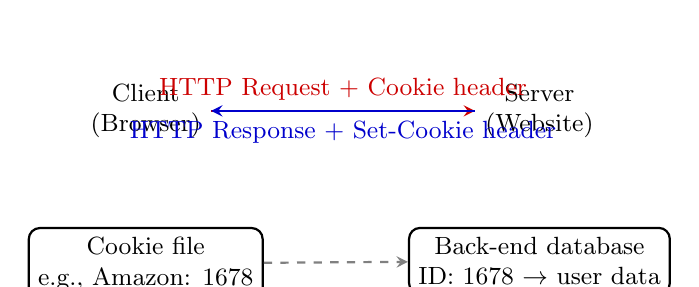
\begin{tikzpicture}[>=stealth, node distance=5cm, thick, font=\small]
        % Nodes
        \node (client) [align=center] {Client \\ (Browser)};
        \node (server) [right of=client, align=center] {Server \\ (Website)};

        % Cookie file and DB
        \node[below=1cm of client] (cookiefile) [draw, rounded corners, align=center] {Cookie file\\ e.g., Amazon: 1678};
        \node[below=1cm of server] (database) [draw, rounded corners, align=center] {Back-end database\\ ID: 1678 $\rightarrow$ user data};

        % Arrows
        \draw[->, color=red!80!black] (client) -- node[above]{HTTP Request + Cookie header} (server);
        \draw[->, color=blue!80!black] (server) -- node[below]{HTTP Response + Set-Cookie header} (client);
        \draw[->, dashed, color=gray] (cookiefile) -- (database);

    \end{tikzpicture}
    \caption{Cookie-based State Management: How client and server maintain user state using cookies.}
    \label{fig:cookie_state}
\end{figure}


\subsection{Cookie Applications and Privacy}
\begin{itemize}
    \item \textbf{Uses:} Authorization, shopping carts, recommendations, user sessions
    \item \textbf{Privacy concerns:}
          \begin{itemize}
              \item Sites learn about user behavior
              \item Third-party persistent cookies track across multiple sites
              \item Common identity tracking
          \end{itemize}
\end{itemize}

\textcolor{orange}{[Mnemonic: Cookies have 4 C's: Client, Cache, Communication, Control]}
\textcolor{blue}{[Summary: Cookies overcome HTTP's stateless nature by storing user-specific data, enabling personalized experiences but raising privacy concerns.]}

\section{Web Caching and Performance}

\subsection{Web Caches (Proxy Servers)}
\begin{itemize}
    \item \textbf{Goal:} Satisfy client requests without origin server involvement
    \item Browser configured to point to local web cache
    \item Cache acts as both client and server
\end{itemize}

\textbf{Cache Operation:}
\begin{enumerate}
    \item Browser sends request to cache
    \item If object in cache: return to client
    \item Else: request from origin server, cache object, return to client
\end{enumerate}

\subsection{Cache Control Headers}
\begin{itemize}
    \item \textbf{Cache-Control: max-age=<seconds>:} Object caching duration
    \item \textbf{Cache-Control: no-cache:} Do not cache object
\end{itemize}

\subsection{Benefits of Web Caching}
\begin{itemize}
    \item Reduce client response time (cache closer to client)
    \item Reduce traffic on institution's access link
    \item Enable efficient content delivery for providers
\end{itemize}

\section{Caching Performance Analysis}

\subsection{Base Scenario}
\begin{itemize}
    \item Access link rate: 1.54 Mbps
    \item RTT to server: 2 seconds
    \item Web object size: 100K bits
    \item Request rate: 15 requests/second
    \item Data rate to browsers: 1.50 Mbps
\end{itemize}

\textbf{Performance without Cache:}
\begin{itemize}
    \item Access link utilization: 0.97 (97\%)
    \item LAN utilization: 0.0015
    \item End-end delay: 2 sec + minutes + microseconds
\end{itemize}
sdf
\subsection{Option 1: Faster Access Link}
\begin{itemize}
    \item Upgrade to 154 Mbps access link
    \item Access link utilization: 0.0097 (0.97\%)
    \item Cost: Expensive
\end{itemize}

\subsection{Option 2: Web Cache}
\begin{itemize}
    \item Install local web cache
    \item Cost: Cheap
\end{itemize}

\textbf{Performance with Cache (40\% hit rate):}
\begin{itemize}
    \item 40\% requests served by cache (low msec delay)
    \item 60\% requests served by origin
    \item Access link data rate: $0.6 \times 1.50 \text{ Mbps} = 0.9 \text{ Mbps}$
    \item Access link utilization: $0.9 / 1.54 = 0.58$
    \item Average end-end delay:
          \[
              \begin{aligned}
                  \text{Delay} & = 0.6 \times (\text{delay from origin}) + 0.4 \times (\text{delay from cache}) \\
                               & = 0.6 \times 2.01 + 0.4 \times (\text{msecs}) \approx 1.2 \text{ seconds}
              \end{aligned}
          \]
\end{itemize}

\textcolor{blue}{[Summary: Web caching dramatically improves performance by serving content locally, reducing both response time and network traffic compared to upgrading infrastructure.]}

\section{Advanced HTTP Features}

\subsection{Conditional GET}
\begin{itemize}
    \item \textbf{Goal:} Avoid sending object if cache has up-to-date version
    \item Client includes: \texttt{If-modified-since: <date>}
    \item Server responses:
          \begin{itemize}
              \item \textbf{304 Not Modified:} Cached copy is current
              \item \textbf{200 OK:} Object modified, new version sent
          \end{itemize}
\end{itemize}

\subsection{HTTP/2}
\begin{itemize}
    \item \textbf{Key goal:} Decrease delay in multi-object requests
    \item Improvements over HTTP 1.1:
          \begin{itemize}
              \item Object transmission based on client-specified priority (not FCFS)
              \item Push unrequested objects to client
              \item Divide objects into frames
              \item Mitigate Head-of-Line (HOL) blocking
          \end{itemize}
\end{itemize}

\subsubsection{HOL Blocking Mitigation}
\begin{itemize}
    \item \textbf{HTTP 1.1:} Objects delivered in request order
          \begin{itemize}
              \item Small objects wait behind large objects
          \end{itemize}
    \item \textbf{HTTP/2:} Objects divided into frames, transmission interleaved
          \begin{itemize}
              \item Small objects delivered quickly
              \item Large objects slightly delayed
          \end{itemize}
\end{itemize}

\subsection{HTTP/3}
\begin{itemize}
    \item \textbf{Limitations of HTTP/2:}
          \begin{itemize}
              \item Single TCP connection means packet loss stalls all objects
              \item Browsers open multiple parallel TCP connections
              \item No security over vanilla TCP
          \end{itemize}
    \item \textbf{HTTP/3 improvements:}
          \begin{itemize}
              \item Adds security
              \item Per-object error and congestion control over UDP
              \item More pipelining capabilities
          \end{itemize}
\end{itemize}

\textcolor{teal}{[Concept Map:
            \begin{itemize}
                \item HTTP 1.0 → Non-persistent → High latency
                \item HTTP 1.1 → Persistent → Reduced connections
                \item HTTP/2 → Frame multiplexing → HOL blocking mitigation
                \item HTTP/3 → UDP-based → Per-object control + security
            \end{itemize}
        ]}

\end{document}


\end{document}